\begin{flushright} {\tiny {\color{gray} (tikz\_dssy2D.tex)}} \end{flushright}
%~~~~~~~~~~~~~~~~~~~~~~~~~~~~~~~~~~~~~~~~~~~~~~~~~~~~~~~~~~~~~~~~~~~~~~~~~~~~~~~~~~~~~~~~~~~~~~~~~~

\begin{center}
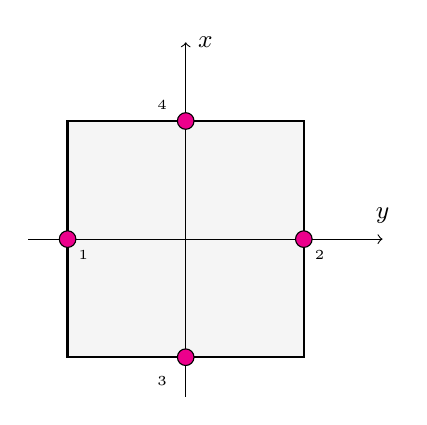
\begin{tikzpicture}
%\draw[step=1cm,gray,very thin] (0,0) grid (8,8); %background grid

\draw[thick,fill=gray!8] (1,1) -- (4,1) -- (4,4) -- (1,4) -- cycle;

\node[] at (1.2,2.3) {\tiny 1};
\node[] at (4.2,2.3) {\tiny 2};
\node[] at (2.2,.7) {\tiny 3};
\node[] at (2.2,4.2) {\tiny 4};

\draw[->] (0.5,2.5)--(5,2.5);
\draw[->] (2.5,0.5)--(2.5,5);

\draw[black,fill=magenta] (1,2.5)   circle (3pt);
\draw[black,fill=magenta] (4,2.5)   circle (3pt);
\draw[black,fill=magenta] (2.5,1)   circle (3pt);
\draw[black,fill=magenta] (2.5,4)   circle (3pt);

\node[] at (5,2.8) {\small $y$};
\node[] at (2.75,5) {\small $x$};
\end{tikzpicture}
\end{center}


